\startchapter{AI-driven Software Engineering}
\label{chapter:Exp}

The current approaches focus on programming-in-the-small \cite{DeRemer1976} i.e, on individual lines of code. 
Code language models have focused (effectively!) on source code as natural language~\cite{natural}.
This models the software development task as predicting the next token or series of tokens.
As Copilot's webpage says, the aim for Copilot is to produce ``safe and effective code [with] suggestions for whole lines or entire functions'' as ``your AI pair programmer''~\cite{Copilot-web}. 
Thus support from language models is currently focused on software \textit{programming}, rather than software \emph{engineering} (in-the-large). 
% \neil{wut? --D} 
% But there are areas of code suggestions that are not easily fixable or at least, not detectable efficiently before training or recommendation is required, at the time-scale of code completion (which we assume is nearly instantaneous, as evidenced by how existing autocomplete editors work.)

What might AI support for these more complex software engineering challenges require? 
We present a simple taxonomy in Figure \ref{fig:levels}, modeled on the ideas in the SAE taxonomy and Koopman's extension for self-driving vehicles (Fig. \ref{fig:koopman_pyramid}), as one way of thinking about this question. 

\section{Taxonomy}
\label{taxonomy}
Our taxonomy is a software abstraction hierarchy where ``basic programming functionality'' such as code compilation and syntax checking is the lowest abstraction level,
Software architecture analysis and design are at the highest abstraction level.
As we ascend the levels, just as with Koopman's pyramid in figure \ref{fig:koopman_pyramid}, 
software challenges rely more on human input and become more difficult to automate (e.g., crafting design rules vs. following syntax rules).

Figure~\ref{fig:taxonomy} shows the taxonomy of autonomy levels for \cct{}. The more abstract top levels depend on the resolution of the lower ones. As we move up the hierarchy, we require more human oversight of the AI; as we move down the hierarchy, rules for detecting problems are easier to formulate. Green levels are areas where \cct{} like Copilot works reasonably well, while red levels are challenging for Copilot based on tests shown in Chapter~\ref{chapter:methodology}.

\begin{figure}[hbt!]
    \centering
    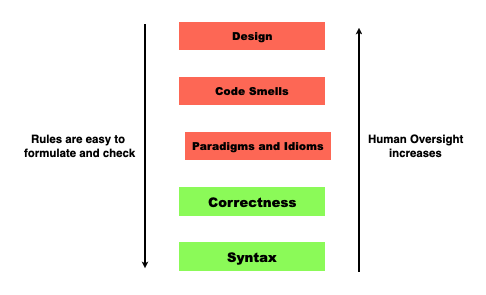
\includegraphics[width=\linewidth]{Figures/taxonomy.png}
    \caption{Hierarchy of software abstractions. Copilot cleared all green levels and struggled in red levels}
    \label{fig:taxonomy}
\end{figure}

Based on our tests with Copilot shown in chapter~\ref{chapter:methodology}, Copilot was able to generate syntactically correct code that solves the given programming task in the coding scenario~(shown in ~\repl{}).
This functionality covers the syntax and the correctness level in our software abstraction hierarchy.
As a result, Copilot stands at the correctness level of our taxonomy. 

The challenges further up the hierarchy are nonetheless more important for software quality attributes (QA)~\cite{Ernst2017} and for a well-engineered software system.
For example, an automated solution suggested by \cct{} to the top level of the taxonomy would be able to follow heuristics to engineer a well-designed software system, which would be easy to modify and scale to sudden changes in use.
\subsection{Paradigms and Idioms}
Paradigms and idioms are our taxonomy's third level of software abstraction. 
This level requires the code suggested by \cct{} to satisfy all the previous levels of abstractions and use common paradigms and language idioms in its code suggestions. 
These include common practices of solving a programming task. 

Returning to our running example of performing a sorting operation on a list of numbers. 
To satisfy this level of abstraction, \cct{} should suggest a syntactically correct list sorting code, using idiomatic ways in its code suggestions, like the Pythonic way of swapping items in a list~(line 5 in figure~\ref{fig:idioms}), As opposed to suggesting non-idiomatic approaches like creating another temporary variable to swap items in a list shown in correctness level~(figure~\ref{fig:correctness}).

Figure~\ref{fig:idioms} shows the sorting example and the Python code suggestions from \cct{} at this abstraction level.

\begin{figure}[hbt!]
    \centering
\begin{tcolorbox}[title=Idioms level suggestion for sort routine,boxsep=.15mm]
    %https://tex.stackexchange.com/questions/337909/tcolorbox-tcbline-style
\textbf{Human Input:}
\begin{lstlisting}[language={Python}]
# sorting a list
arr = [2,4,1,3,7,5]
\end{lstlisting}
\tcbline
\textbf{\cct{} suggestion:}
\begin{lstlisting}[language={Python}]
n = len(arr)
for i in range(n):
	for j in range(n-1):
		if arr[j] > arr[j+1]:
			arr[j], arr[j+1] = arr[j+1], arr[j]
print(arr)
\end{lstlisting}
\end{tcolorbox}
    \caption{Code suggestion of \cct{} at paradigms and idioms level.}
    \label{fig:idioms}
\end{figure}

The goal of this software abstraction level in the taxonomy is for \cct{} to detect and use commonly known idiomatic approaches and paradigms that occur in public code in its suggestions for suggesting code to solve a programming task.

The capabilities required by \cct{} to satisfy paradigms and idioms level of software abstraction are as follows:
\begin{enumerate}
    \item Identify common patterns like paradigms and language idioms in public code repositories~(training data).
    \item Use paradigms and language idioms in suggesting solutions for a programming task.
    \item Satisfy requirements of all the levels below paradigms and idioms in our taxonomy.
\end{enumerate}


\section{Code Review Best Practices}
We considered best practices for code review in JavaScript development. 
This aligns with the Code Smell level (middle tier) in our taxonomy. 
To ground our practices we relied on the AirBNB JavaScript coding style guide~\cite{airbnb_code}, a widely used coding style and code review standard. 
The AirBNB standard contains a variety of best practices. 
To scope our approach, we chose practices that were closer to the the design level of our taxonomy, rather than the code level (e.g., trailing comma use in Javascript).

% For example, in JavaScript, callback api was used in the past to achieve concurrency which were replaced by promises. We checked if copilot suggests code which is specifically mentioned in the JavaScript documentation as a bad practice or an anti-pattern. Bad Practices in using promises for asynchronous JavaScript like not returning promises after creation, forgetting to terminate chains without catch statement, which are explained in documentation\footnote{\url{https://developer.mozilla.org/en-US/docs/Web/JavaScript/Guide/Using_promises}} and StackOverflow\footnote{\url{https://stackoverflow.com/questions/30362733/handling-errors-in-promise-all/}} are not known to copilot and suggested code with those common anti-patterns as they occur more frequently in copilot training data.

\noindent\textbf{Method:} We chose 5 JavaScript coding standards from the AirBNB JavaScript coding style guide~\cite{airbnb_code}. We considered it a match if Copilot suggested the recommended way in the first 2 suggestions, but note if the recommended way appeared any of the top 10 suggestions. 
Below is the list of five best practices we tested:
% \neil{i think a quick list listing the chosen standards would help, alongside the place the suggestion occurred (e.g.).}

\begin{itemize}
    \item Practice 1: Object Shorthand: Usage of object method shorthand (no suggestion matched)
    \item Practice 2: Array Creating Constructor (place: 6th)
    \item Practice 3: Copying Array Contents (no suggestion matched)
    \item Practice 4: Logging a Function (no suggestion matched)
    \item Practice 5: Exporting a Function (no suggestion matched)
\end{itemize}

Copilot failed to suggest the recommended way for all five standards we tested, i.e, Copilot did not have the recommended way in its top two suggestions. Only 1 out of 5 standards had the recommended way in the top 10 suggestions. 

Below is an example of logging a function (Practice 4). 
We first show the user input that triggers Copilot, the top suggestion by Copilot (i.e. model output) and the recommended way suggested by the AirBNB coding style guide~\cite{airbnb_code}.

\begin{tcolorbox}[title=Logging a Function,boxsep=.5mm]
    %https://tex.stackexchange.com/questions/337909/tcolorbox-tcbline-style
\textbf{Human Input:}
\begin{lstlisting}[language=JavaScript]
// logging function

class foo {
    bar ()
\end{lstlisting}
\tcbline
\textbf{Copilot Suggestion:}
\begin{lstlisting}[language=JavaScript]
{
    console.log('bar');
    }
}
\end{lstlisting}
\tcbline
\textbf{Ideal way\footnote{source~\cite{airbnb_code}}:}
\begin{lstlisting}[language=JavaScript]
class foo {
    bar (){ 
    console.log(this.bar) ;
}}
\end{lstlisting}
\end{tcolorbox}

\section{Design Smells}
Currently, Copilot does not support multi-file input, So it is not possible to evaluate its design suggestions, as software development process may include multiple folders with a file structure. 
Making Code completion tools adapt their suggestions to context specific issues such as variable naming conventions and formatting would be challenging as the existing guidelines are not standard in this space and mostly depend on context, The training dataset for AI driven development should also include rules such as idioms, best practices before tackling design level problems.
% Design smells or arch smells (Tushar Sharma)
\section{Chapter Summary}
In summary, we start this chapter by showing the methodology used in addressing \textbf{RQ-1.2} (How do \cct{} manage to suggest non-smelly code?). We first introduced the study setup with the input to Copilot and how it was restricted to deriving the best practice from the input and how the suggestions from Copilot were evaluated. We sampled best practices from AirBNB JavaScript coding style guide~\cite{airbnb_code}, and then compared it against Copilot suggestions. Based on results shown in Table~\ref{tab:all_bp}, Copilot struggles to suggest the best practices from widely used coding standards in its suggestions. 

In this chapter, we showed that Copilot struggles to detect and follow coding style guides  present in public repositories of GitHub and always suggest code that follows those coding style guides. The ideal behavior of \cct{} like Copilot in solving this problem is to detect the coding style guideline from existing code in the project and always suggest code that follows the guideline.

In the next chapter (chapter~\ref{chapter:framework}), we illustrate our taxonomy inspired from autonomous driving levels on the software abstraction hierarchy in \AISE{}, and delineate where \cct{} are currently best able to perform, and where more complex software engineering tasks overwhelm them.